\section{Aplicación móvil}

Un completo análisis para el desarrollo de la aplicación móvil se incluye como Anexo de este documento. Esta sección pretende mostrar los resultados de la implementación realizada.

La aplicación permitirá al usuario registrar ciertos datos de los pacientes, incluyendo el número telefónico asociado a la tarjeta SIM ubicada en el módulo 4G. Una vez registrado un usuario, podrá consultar y editar esta información. \\

Al consultar los registros de los signos vitales, se recuperará la información de los mensajes de texto y de la base de datos para mostrar la información actualizada de estas mediciones. \\

Estas funcionalidades se muestran en la figura \ref{fig:casosUso:AplicacionResumen}

\begin{figure}[htpb!]
	\begin{center}
		\fbox{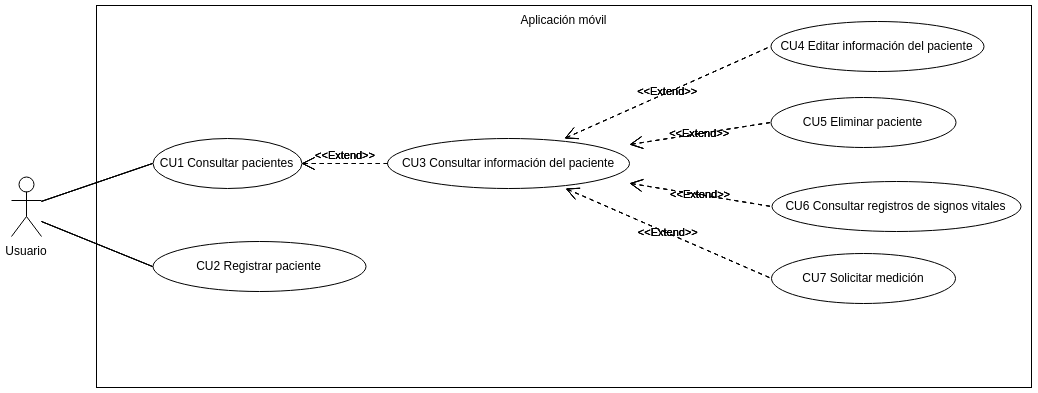
\includegraphics[width=1\textwidth]{ModeloComportamiento/imagenes/CasosUso_Usuario.png}}
		\caption{Diagrama de casos de uso del módulo Aplicación Móvil. \label{fig:casosUso:AplicacionResumen}}
	\end{center}
\end{figure}

\subsection{Diseño de pantallas}


PANTALLAS Y FUNCIONALIDAD